\documentclass[11pt]{article}
\pdfpxdimen=1in
\divide\pdfpxdimen by 300
 
\usepackage[latin1]{inputenc}
\usepackage[T1]{fontenc}
\usepackage[english]{babel}
\usepackage{mathtools, bm}
\usepackage{amssymb, bm}
\usepackage{float}

\usepackage{caption} % to center captions
\usepackage{subcaption} % subcaption for figures side by side

\usepackage{booktabs} % for super cool table
\usepackage[table,xcdraw]{xcolor}  % to put color in tables
\usepackage{tcolorbox} % add box
\usepackage{commath} % for absolute values

\usepackage[parfill]{parskip}
\usepackage{graphicx}
\usepackage{hyperref}
\usepackage[top=0.8in, bottom=0.8in, left=1in, right=1in]{geometry}
\usepackage{listings}
\usepackage{multirow}


\renewcommand\thesubsection{\thesection.\arabic{subsection}} % Subsection starting with A, B, ...

\renewcommand\thefigure{\thesubsection.\arabic{figure}}

\newcommand{\horrule}[1]{\rule{\linewidth}{#1}} % Create horizontal rule command with 1 argument of height

\numberwithin{figure}{section} % to have per-section figure numbering

\title{	
\normalfont \normalsize 
\textsc{Master MVA \\
Reinforcement Learning} \\ [20pt]
\horrule{0.5pt} \\[0.2cm] % Thin top horizontal rule
\textbf{TP 2}: The Exploration-Exploitation Dilemma \\
\horrule{2pt} \\[0.3cm] % Thick bottom horizontal rule
}

\author{Victor Busa \\
   \texttt{victor.busa@ens-paris-saclay.fr}}

\date{\normalsize\today}

\begin{document}

\maketitle

\section{Stochastic Multi-Armed Bandits on Simulated Data}
\subsection{Bernoulli bandit models}
\paragraph{Comparison between UCB1 and NAIVE}

I used two different Multi-Armed Bandit problems. One complex problem with complexity $C_1(p) = 273.69$ and an easy problem whose complexity is $C_2(p) = 1.90$. All the arms are drawn from a Bernoulli distributions and the mean parameter of each arm is detailed in Table ~\ref{table:complex_ber} and Table ~\ref{table:easy_ber} below.

\begin{table}[h]
\centering
\begin{tabular}{|c|c|c|l|l|l|l|}
\hline
 & \textbf{Arm1} & \textbf{Arm2} & \textbf{Arm3} & \textbf{Arm4} & \textbf{Arm5} & \textbf{Arm6} \\ \hline
Mean & 0.2 & 0.65 & \textbf{0.797} & 0.794 & 0.795 & \textbf{0.797} \\ \hline
\end{tabular}
\caption{Mean parameter of each Bernoulli arms for the complex problem: $C_1(p) = 273.69$}
\label{table:complex_ber}
\end{table}

\begin{table}[h]
\centering
\begin{tabular}{|c|c|c|l|}
\hline
 & \textbf{Arm1} & \textbf{Arm2} & \textbf{Arm3} \\ \hline
Mean & 0.3 & \textbf{0.8} & 0.4 \\ \hline
\end{tabular}
\caption{Mean parameter of each Bernoulli arms for the easy problem: $C_2(p) = 1.90$}
\label{table:easy_ber}
\end{table}

Figure ~\ref{fig:UCB1_v_NAIVE_complex} and Figure ~\ref{fig:UCB1_v_NAIVE_easy} depict the observed cumulated regret averaged over $50$ simulations of $60000$ episodes each for \texttt{UCB1} with different values of $\alpha$ and the \texttt{NAIVE} algorithm for respectively the complex and the easy problem. We can see that, on average \texttt{UCB1} outperforms the \texttt{NAIVE} implementation on the easy problem as its regret is lower than the naive regret. Moreover, if we tune correctly the parameter $\alpha$, \texttt{UCB1} highly outperforms the \texttt{NAIVE} algorithm on the easy problem as we can see for $\alpha = 0.5$. \\
\\
For the complex problem we can see that \texttt{UCB1} still outperforms the \texttt{NAIVE} implementation and achieve the best results for low values of $\alpha$. For $\alpha = 2$ the performance of \texttt{UCB1} looks very similar to the performance of the \texttt{NAIVE} implementation. This is due to the fact that the parameter $\alpha$ control the rate of exploration. Hence a higher $\alpha$ will favors exploration over exploitation. Large value of $\alpha$ will then decrease the performance of the \texttt{UCB1} algorithm. \\
\\
\textbf{Note}: Intuitively, we might think that for the easy problem the \texttt{NAIVE} implementation and the \texttt{UCB1} implementation should behave in the same manner. Actually the bad performance of the \texttt{NAIVE} algorithm comes from the fact that if at the initialization we draw $[1,0,1]$, i.e a reward of 1 for $Arm_1$, 0 for $Arm_2$ and 1 for $Arm_3$ then we will subsequently not drawn the \textbf{second Arm} while it is the best in our example as $mean(Arm_2)=0.8$. \texttt{UCB1} doesn't have this drawback as it balances between exploitation and exploration through the use of the $\alpha$ parameter.

\begin{figure}[H]
		\centering
		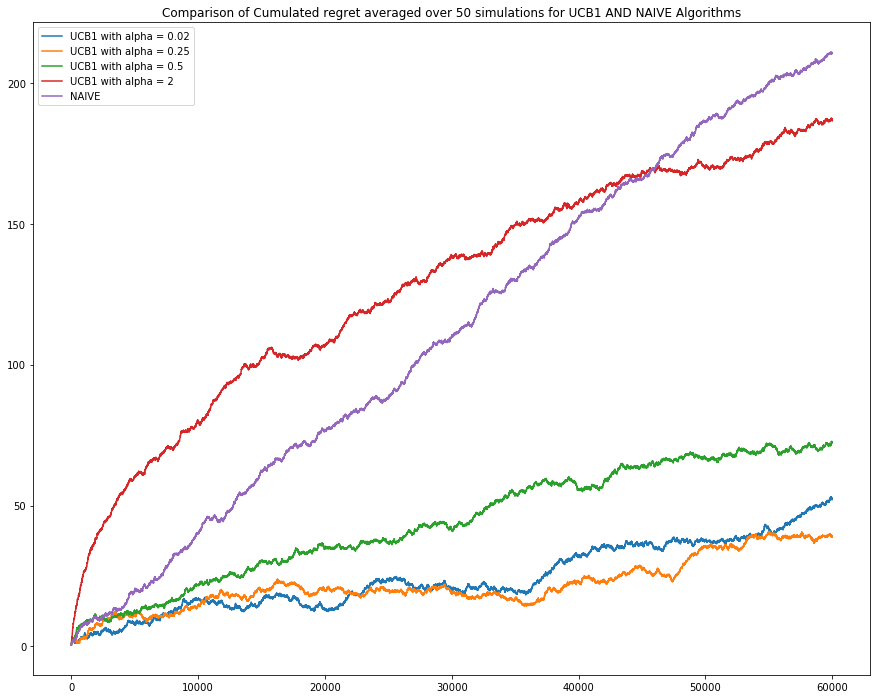
\includegraphics[width=1\linewidth]{images/preli_complex}
		\caption{Cumulated regret averaged over 50 simulations of 60 000 episodes each for \texttt{UCB1} and \texttt{NAIVE} for different values of $\alpha$ on the complex problem}
		\label{fig:UCB1_v_NAIVE_complex}
\end{figure}

\begin{figure}[H]
		\centering
		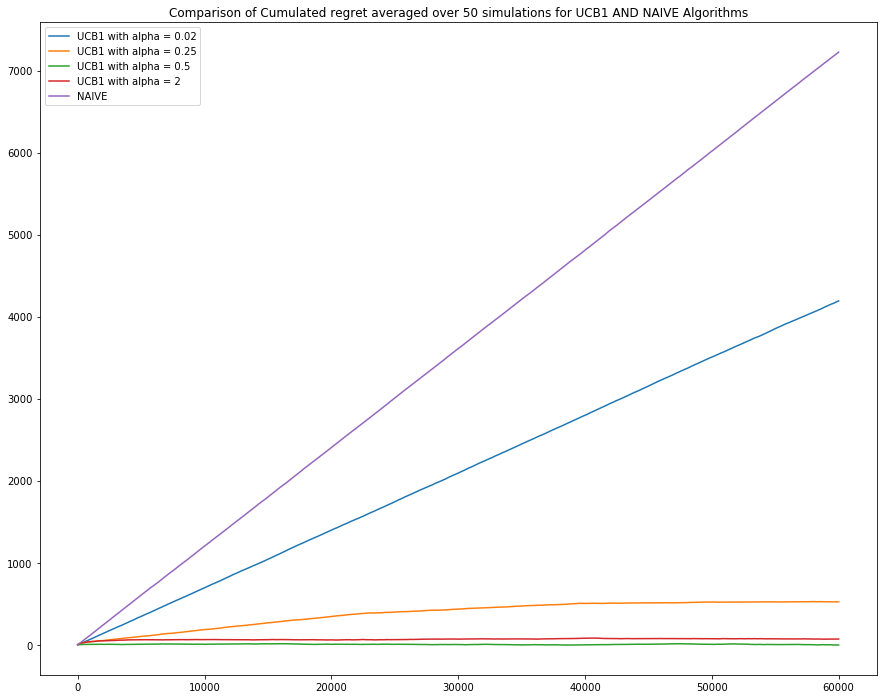
\includegraphics[width=1\linewidth]{images/preli_easy}
		\caption{Cumulated regret averaged over 50 simulations of 60 000 episodes each for \texttt{UCB1} and \texttt{NAIVE} for different values of $\alpha$ on the easy problem}
		\label{fig:UCB1_v_NAIVE_easy}
\end{figure}


\paragraph{Q1: Comparison Between Thompson Sampling and UCB1}\mbox{}\\
\textbf{Problem 1} : 3 Bernoulli with parameters 0.3, 0.8 and 0.4 and complexity $C = 1.91$ \\
\textbf{Problem 2} : 4 Bernoulli with parameters 0.33, 0.34, 0.36, 0.35 and complexity $C = 83.9$

For easy Multi-Armed Bandit problems and for a well-suited value of $\alpha$,  on average, \texttt{UCB1} algorithm outperforms the \texttt{Thompson Sampling} algorithm. The Figure ~\ref{fig:easy_ucb_v_ts} depicts the averaged cumulated regret computed over 500 simulations of 5000 episodes with $\alpha = 0.5$ for \textbf{Problem 1}.

\begin{figure}[H]
    \centering
    \begin{subfigure}{.5\textwidth}
        \centering
        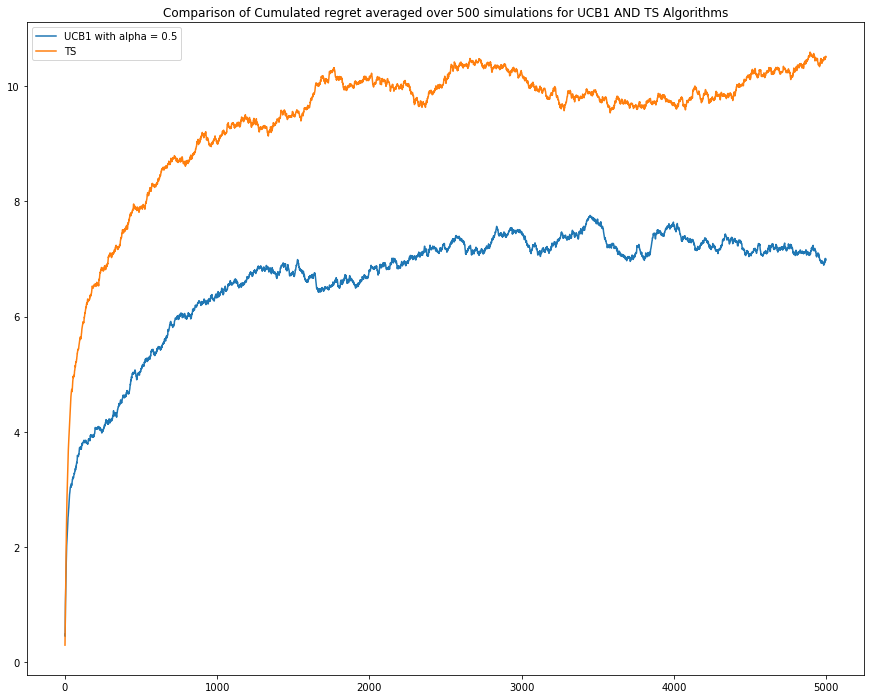
\includegraphics[width=1\linewidth]{images/easy_ucb_v_ts_nolr}
        \caption{First run without Lai Robbins bound}
        \label{fig:easy_without_lr}
    \end{subfigure}%
    \begin{subfigure}{.5\textwidth}
        \centering
        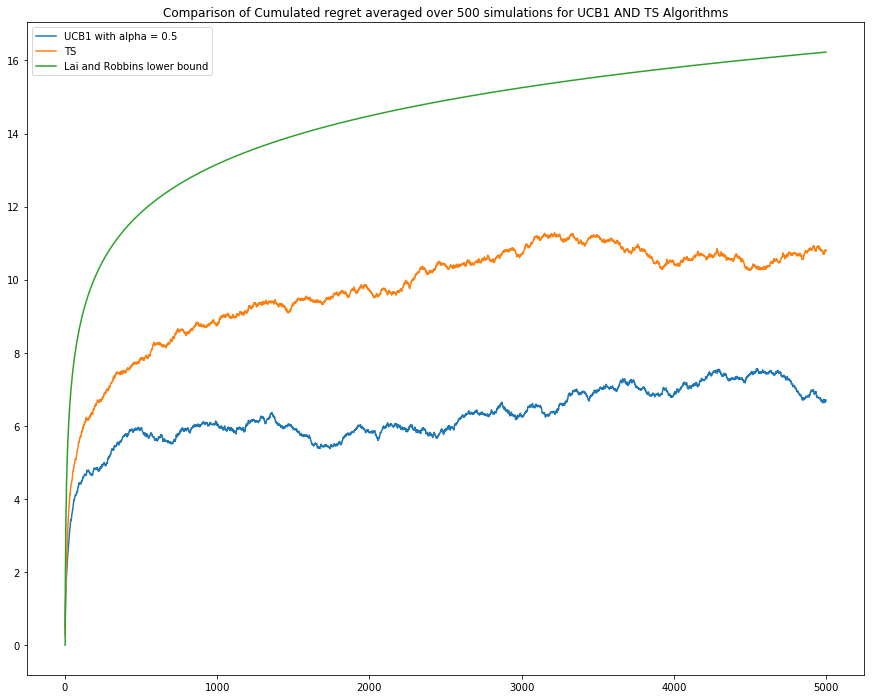
\includegraphics[width=1\linewidth]{images/easy_ucb_v_ts}
        \caption{Second run with Lai Robbins bound}
        \label{fig:easy_lr}
    \end{subfigure}
		\caption{Averaged cumulated reward over 500 simulations for \texttt{UCB1} (Blue curve) and \texttt{Thompson Sampling} (Orange curve) on Problem 1}
\label{fig:easy_ucb_v_ts}
\end{figure}

For complex problems such as \textbf{Problem 2}, \texttt{UCB1} still slightly performs better than \texttt{Thompson Sampling} for well-suited value of $\alpha$. What is striking is the fact that the Lai \& Robbins lower bound appears to be above both curves. This can be explained by the fact that the Lai \& Robbins bound is an \textbf{asymptotic bound} and by the fact that the bound doesn't hold for \textbf{multiparametric} distributions.

\begin{figure}[H]
    \centering
    \begin{subfigure}{.5\textwidth}
        \centering
        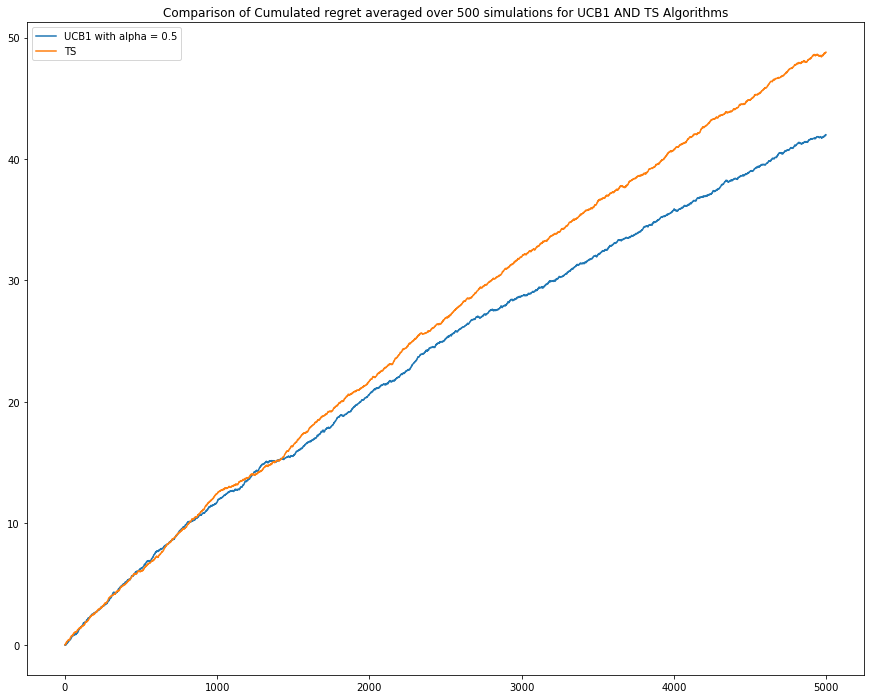
\includegraphics[width=1\linewidth]{images/hard_ucb_v_ts_nolr}
        \caption{First run without Lai Robbins bound}
        \label{fig:hard_without_lr}
    \end{subfigure}%
    \begin{subfigure}{.5\textwidth}
        \centering
        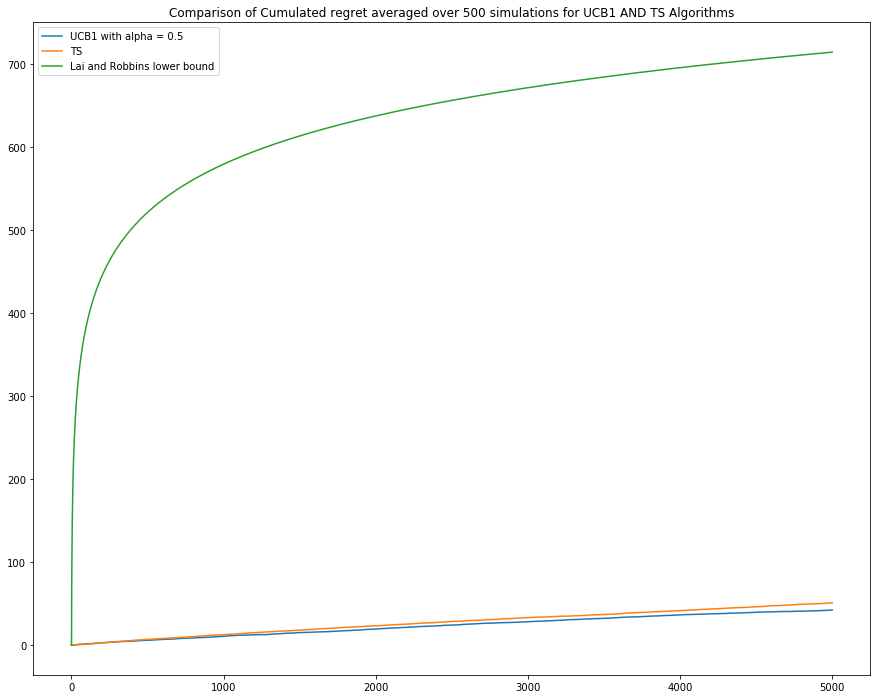
\includegraphics[width=1\linewidth]{images/hard_ucb_v_ts}
        \caption{Second run with Lai Robbins bound}
        \label{fig:hard_lr}
    \end{subfigure}
		\caption{Averaged cumulated regret over 500 simulations for \texttt{UCB1} (Blue curve) and \texttt{Thomson Sampling} (Orange curve) on Problem 2}
\label{fig:hard_ucb_v_ts}
\end{figure}

\subsection{Non-parametric bandits (bounded rewards)}
\paragraph{Q2 Adaptation of Thompson Sampling}\mbox{}\\

We can adapt Thompson Sampling algorithm so that it works for general stochastic bandits. The idea is to performs a Bernoulli trial with success probability $\widetilde{r_t}$ where $\widetilde{r_t}$ is the reward observed at time t from pulling the arm $a_t$. From this Bernoulli trial we observe $r_t \in \{0, 1\}$ and we then proceed by updating $N$ and $S$ based on the traditional Thompson Sampling algorithm.

For this question we consider the model in table ~\ref{table:mab_model}
\begin{table}[H]
\centering
\small
\begin{tabular}{|l|l|l|l|l|l|l|l|l|l|l|l|}
\hline
\textbf{Arm} & 1 & 2 & 3 & 4 & 5 & 6 & 7 & 8 & 9 \\ \hline
\textbf{Type} & exp(2) & exp(3) & exp(4) & exp(5) & beta(3,9) & beta(4,8) & beta(5,7) & beta(6,6) & Ber(0.8) \\ \hline
\textbf{mean} & 0.57 & 0.35 & 0.25 & 0.20 & 0.25 & 0.33 & 0.42 & 0.5 & \textbf{0.65} \\ \hline
\end{tabular}
\caption{Multi-Armed bandit model}
\label{table:mab_model}
\end{table}

For this model we can see on Figure ~\ref{fig:UCB1_v_TS_GEN} that UCB1 outperforms Thompson sampling algorithm for $\alpha = 0.5$.

\begin{figure}[H]
		\centering
		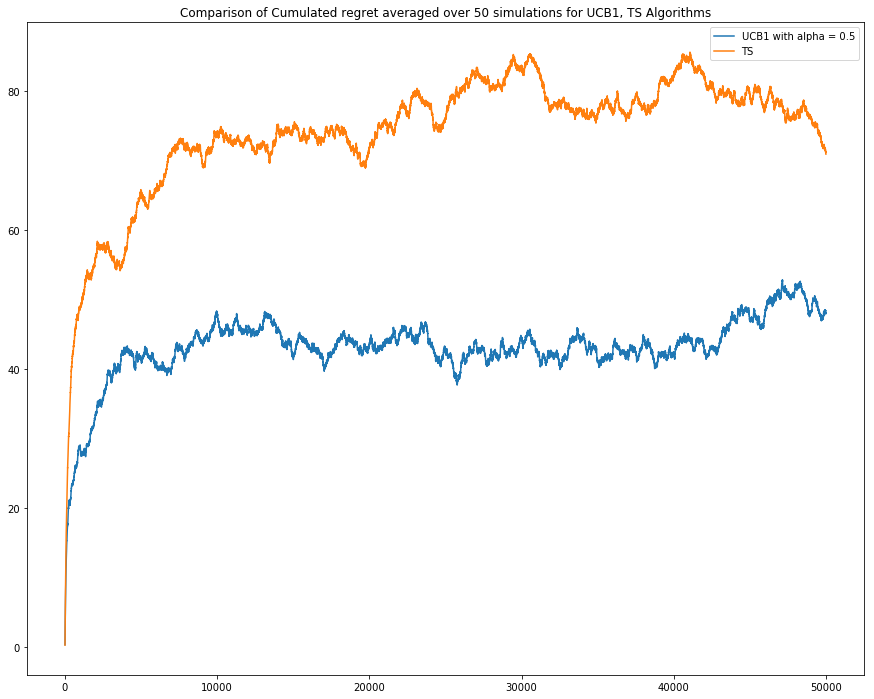
\includegraphics[width=1\linewidth]{images/non_ber_arms}
		\caption{Cumulated regret averaged over 50 simulations of 50 000 episodes each for \texttt{UCB1} and \texttt{Thompson Sampling} for $\alpha = 0.5$}
		\label{fig:UCB1_v_TS_GEN}
\end{figure}


\section{Linear Bandit on Real Data}
I implemented two optimized version of \texttt{linUCB} algorithm (see Python code). The \texttt{linUCB2} implementation is slightly faster but prevent me
from tracing the curve $\norm{\widehat{\theta}_t - \theta^{\star}}_2$ in function of the number of iterations. That is why I choose to use the \texttt{linUCB}
implementation in the remaining part.

I used the following formula to compute $\alpha$:

\begin{align*}
\alpha = \sqrt{\dfrac{1}{2} log \; \dfrac{(2 . T . K)}{\delta}}
\end{align*}

where I choose $\delta = 10^{-3}$,  $T = 6000$ (number of episode) and $K= 207$ (number of arms of the problem). Numerically I have $\alpha = 3.29$. In the remaining experiment
I also set $\lambda = 2$ (regularization hyperparameter), $\epsilon = 0.1$ (for the greedy epsilon algorithm) and I averaged the result over \textbf{20 simulations}. Figure ~\ref{fig:lin_theta} and ~\ref{fig:lin_regret} show the result I obtained for the \textbf{ColdStartMovieLensModel}.

\begin{figure}[H]
    \centering
    \begin{subfigure}{.5\textwidth}
        \centering
        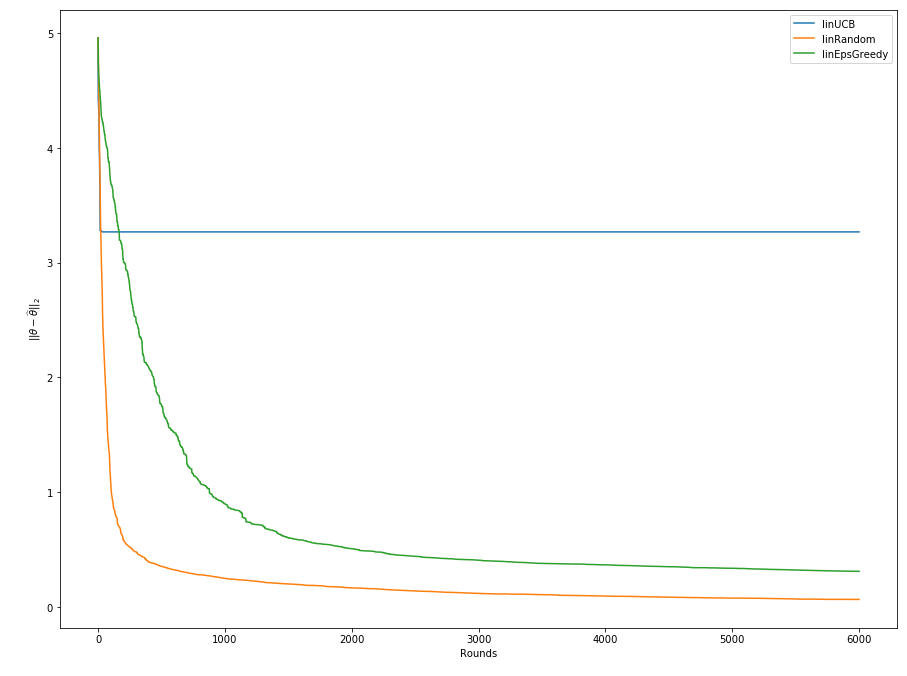
\includegraphics[width=1\linewidth]{images/linUCB_theta}
        \caption{$\norm{\widehat{\theta}_t - \theta^{\star}}_2$ function of the number of iterations}
        \label{fig:lin_theta}
    \end{subfigure}%
    \begin{subfigure}{.5\textwidth}
        \centering
        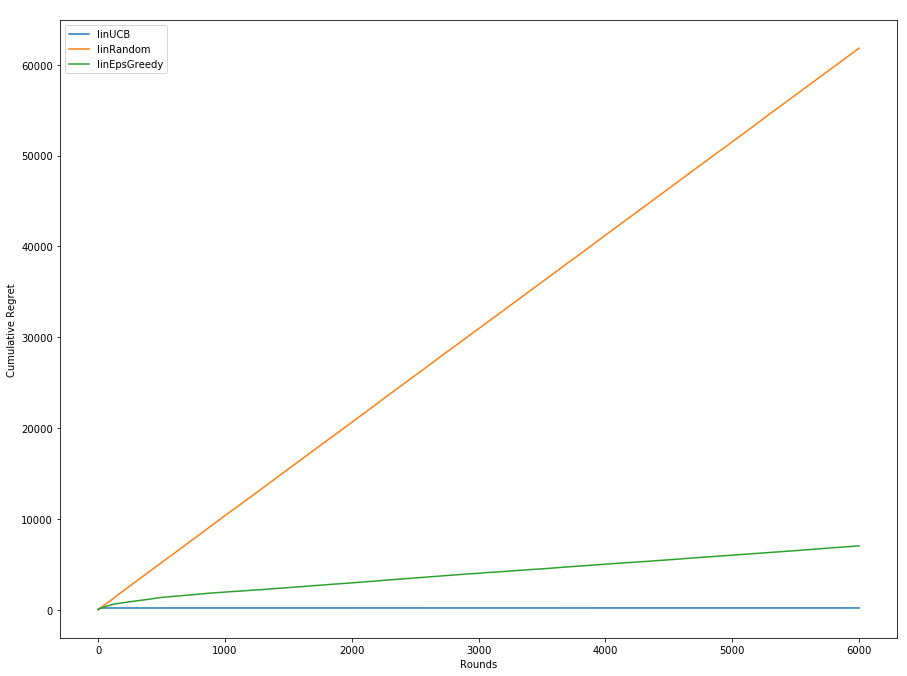
\includegraphics[width=1\linewidth]{images/linUCB_regret}
        \caption{Cumulative averaged regret function of the number of iterations}
        \label{fig:lin_regret}
    \end{subfigure}
		\caption{$\ell_2$ norm of $\widehat{\theta}$ w.r.t the true $\theta$ and Averaged cumulated regret over 20 simulations for \texttt{linUCB} (Blue curve) \texttt{linEpsGreedy} (Green curve) and \texttt{linRandom} (Orange curve) on the ColdStartMovieLensModel model}
\label{fig:lin_graphs}
\end{figure}

I've noticed that for certain value of $\alpha$ and for $\lambda$ fixed, the linUCB algorithm can sometimes give really bad performances. The Table ~\ref{table:alpha_eps_perf} inventories 
how many times we pull the 5 most pulled arms (computed using model.real\_theta) for different values of $\alpha$ and different values of $\epsilon$.

\begin{table}[H]
\centering
\begin{tabular}{|c|l|l|l|l|l|l|}
\hline
\multirow{3}{*}{linUCB} & $\alpha$ = 3.29 & \multicolumn{1}{c|}{(1: 5985)} & \multicolumn{1}{c|}{(8: 1)} & (14: 1) & (29: 1) & (42: 1) \\ \cline{2-7} 
 & $\alpha$ = 0.2 & (29: 5994) & (42: 1) & (166: 1) & (171: 1) & (188: 1) \\ \cline{2-7} 
 & $\alpha$ = 0.5 & (14: 5959) & (29: 32) & (24: 1) & (29:1) & (42: 1) \\ \hline
\multirow{3}{*}{linEpsGreedy} & $\epsilon$ = 0.1 & (1: 5425) & (93: 7) & (102: 7) & (196: 1) & (110: 6) \\ \cline{2-7} 
 & $\epsilon$ = 0.3 & (1: 4240) & (120: 16) & (141: 16) & (164: 16) & (87: 15) \\ \cline{2-7} 
 & $\epsilon$ = 0.01 & (1: 5708) & (42: 234) & (28: 2) & (50: 2) & (154: 2) \\ \hline
\end{tabular}
\caption{($x^{th}$ best arm, number of pulls) for the 5 most pulled arms for different value of $\alpha$ and $\epsilon$ for one simulation of 6000 episodes}
\label{table:alpha_eps_perf}
\end{table}

As we can see on the above table, the linUCB algorithm doesn't work at all for really bad value of $\alpha$. For example we can see that for $\alpha = 0.5$ the
most pulled arm is the $14^{th}$ best-arm with $5959$ pulls and for $\alpha = 0.2$, the most pulled arm is the $29^{th}$ best-arm with $5994$ pulls. We can also clearly see that linEpsGreedy performs the best for low values of $\epsilon$ which is understandable as the higher $\epsilon$ the more the algorithm will explore. But after a certain number of iterations it will know which arm(s) is (are) the best to pick. \\
\\
According to Table ~\ref{table:alpha_eps_perf}, $\alpha = 3.29$, $\epsilon = 0.01$ and $\lambda = 2$ gives us good performance. Taking even higher value for $\alpha$ will give us slightly better performances.

\section{Annexe}
\paragraph{histograms plot for UCB1}\mbox{}\\
I wanted to see what the 3D histograms of cumulated rewards looks like. To do so I used the following complex model ($C = 273.69$):

\begin{table}[H]
\centering
\begin{tabular}{|l|l|l|l|l|l|l|}
\hline
\textbf{Bernoulli arm} & 1 & 2 & 3 & 4 & 5 & 6 \\ \hline
\textbf{mean} & 0.2 & 0.65 & 0.797 & 0.794 & 0.795 & 0.797 \\ \hline
\end{tabular}
\caption{Multi-Armed bandit model}
\label{table:mab_ber}
\end{table}

It appears that \texttt{UBC1} performs the best when $\alpha$ is in the range $[0.2, 0.5]$, while, when $\alpha$ is too low the algorithm will tends to have the same behaviour as the Naive implementation as it can be shown mathematically ($\alpha = 0$is equivalent to the \texttt{NAIVE} algorithm). When $\alpha$ is large \texttt{UCB1} will favor exploration over exploitation and hence the overall performance of \texttt{UCB1} can deplete a lot. The Figure ~\ref{fig:histo_3d} depicts the 3D histograms for $\alpha = 0.2$ and $\alpha = 1$

\begin{figure}[H]
    \centering
    \begin{subfigure}{.5\textwidth}
        \centering
        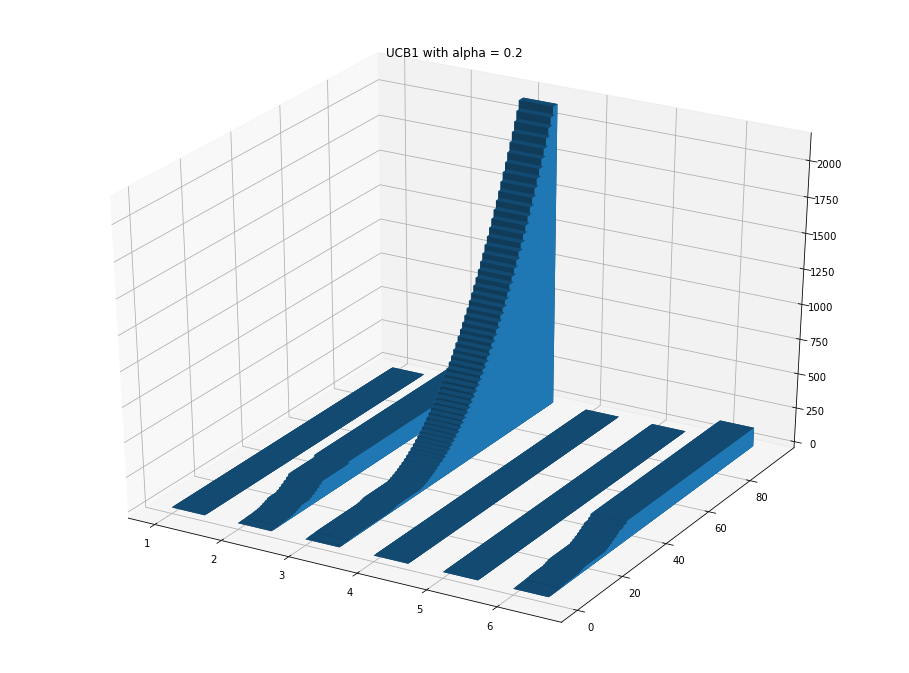
\includegraphics[width=1\linewidth]{images/UCB1_bar_alpha_02}
        \caption{$\alpha = 0.2$}
        \label{fig:bar_02}
    \end{subfigure}%
    \begin{subfigure}{.5\textwidth}
        \centering
        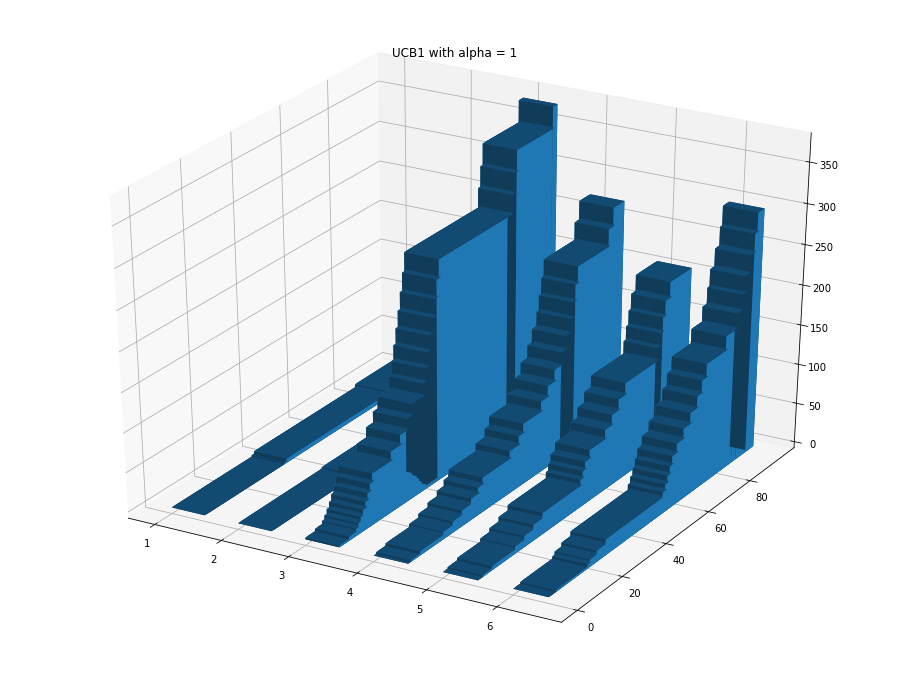
\includegraphics[width=1\linewidth]{images/UCB1_bar_alpha_1}
        \caption{$\alpha = 1$}
        \label{fig:bar_1}
    \end{subfigure}
		\caption{Cumulated reward over 100 episodes for \texttt{UCB1}}
\label{fig:histo_3d}
\end{figure}

\begin{table}[h]
\centering
\begin{tabular}{|c|c|c|l|l|l|l|}
\hline
\textbf{$\alpha$} & \textbf{Arm1} & \textbf{Arm2} & \textbf{Arm3} & \textbf{Arm4} & \textbf{Arm5} & \textbf{Arm6} \\ \hline
0.2 & 1 & 16 & \textbf{65} & 1 & 1 & 16 \\ \hline
1 & \multicolumn{1}{l|}{4} & \multicolumn{1}{l|}{2} & 27 & 23 & 20 & 24 \\ \hline
\end{tabular}
\caption{Number of times each arm is drawn for different value of $\alpha$}
\label{table:nb_drawn}
\end{table}

We can see that for $\alpha = 0.2$ (good choice of $\alpha$) the algorithm quickly detects which arm is the better (Arm3 here) while when $\alpha = 1$ for the same number of iterations the algorithm still struggle to distinguish the best Arm between $Arm_3$, $Arm_4$, $Arm_5$ and $Arm_6$ and for a very good reason their means are really close to each other and the algorithm will tend to explore a lot more.

\end{document}